\documentclass{book}
\usepackage[paperwidth=36in,paperheight=60in,hmargin=0.75in,vmargin=0.75in]{geometry}
\usepackage{graphicx}
\usepackage{ae}

\begin{document}

\setlength{\unitlength}{1in}
\begin{picture}(34.5,58.5){}
\linethickness{0.125in}

%%%%% POSTER BORDER
\put(0,0.0625){\line(1,0){34.4375}}
\put(0,58.375){\line(1,0){34.4375}}
\put(0,0){\line(0,1){58.4375}}
\put(34.375,0){\line(0,1){58.4375}}

%%%%% TITLE TYPE TEXT
\put(0,55.25){
  \makebox(34.25,2.5){
    \centering
    % title
    \fontsize{180}{200}\selectfont Mapping Chaos
  }
}
\put(0,1.5){
  \makebox(34.25,1.5){
    \centering
    % required siggraph name
    \fontsize{100}{120}\selectfont SIGGRAPH 2004
  }
}
\put(0,0.5){
  \makebox(34.25,1){
    \centering
    % required siggraph location
    \fontsize{80}{100}\selectfont Los Angeles, California
  }
}

\linethickness{0.0625in}
%%%%% IMAGE COMPARISON - HDR TECHNIQUES
%%% base image
%\put(0.4375,14.96875){\line(1,0){8.15625}}
%\put(0.4375,23.03125){\line(1,0){8.15625}}
%\put(0.46875,15){\line(0,1){8}}
%\put(8.5625,15){\line(0,1){8}}
\put(0.5,15){
  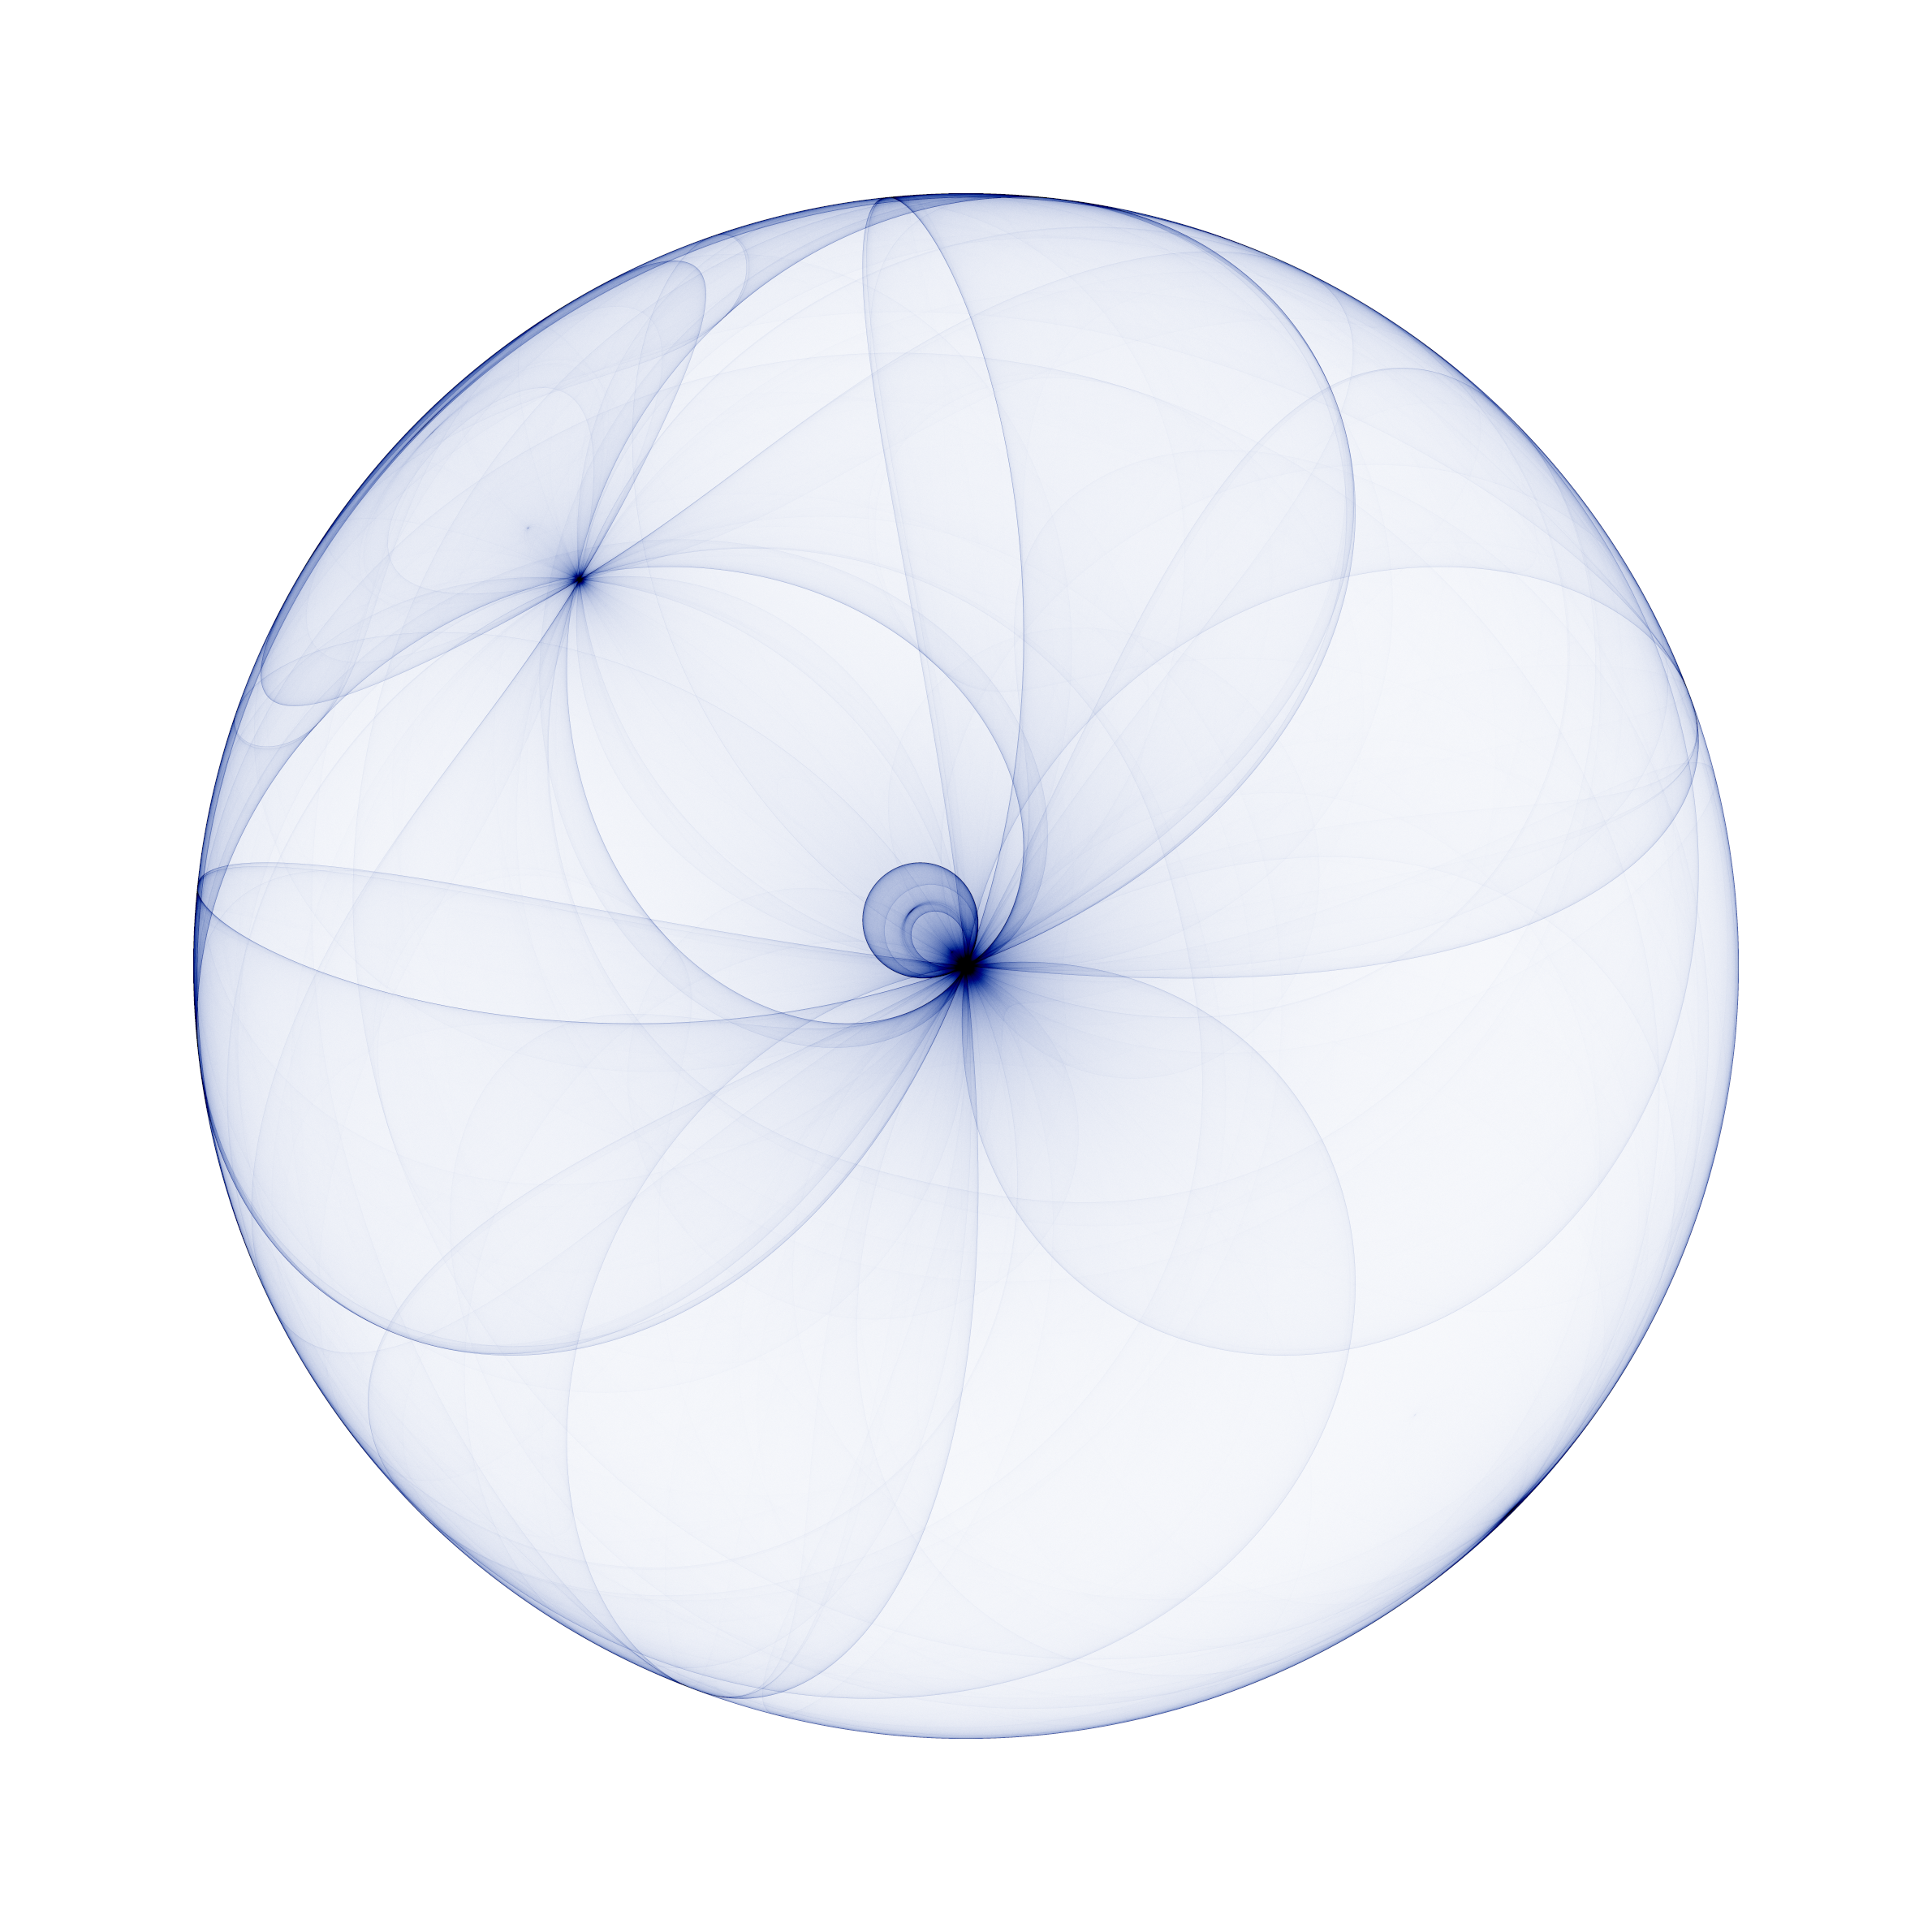
\includegraphics[width=8in]{images/base-large.png}
}

%%% increased exposure
\put(8.5,15){
  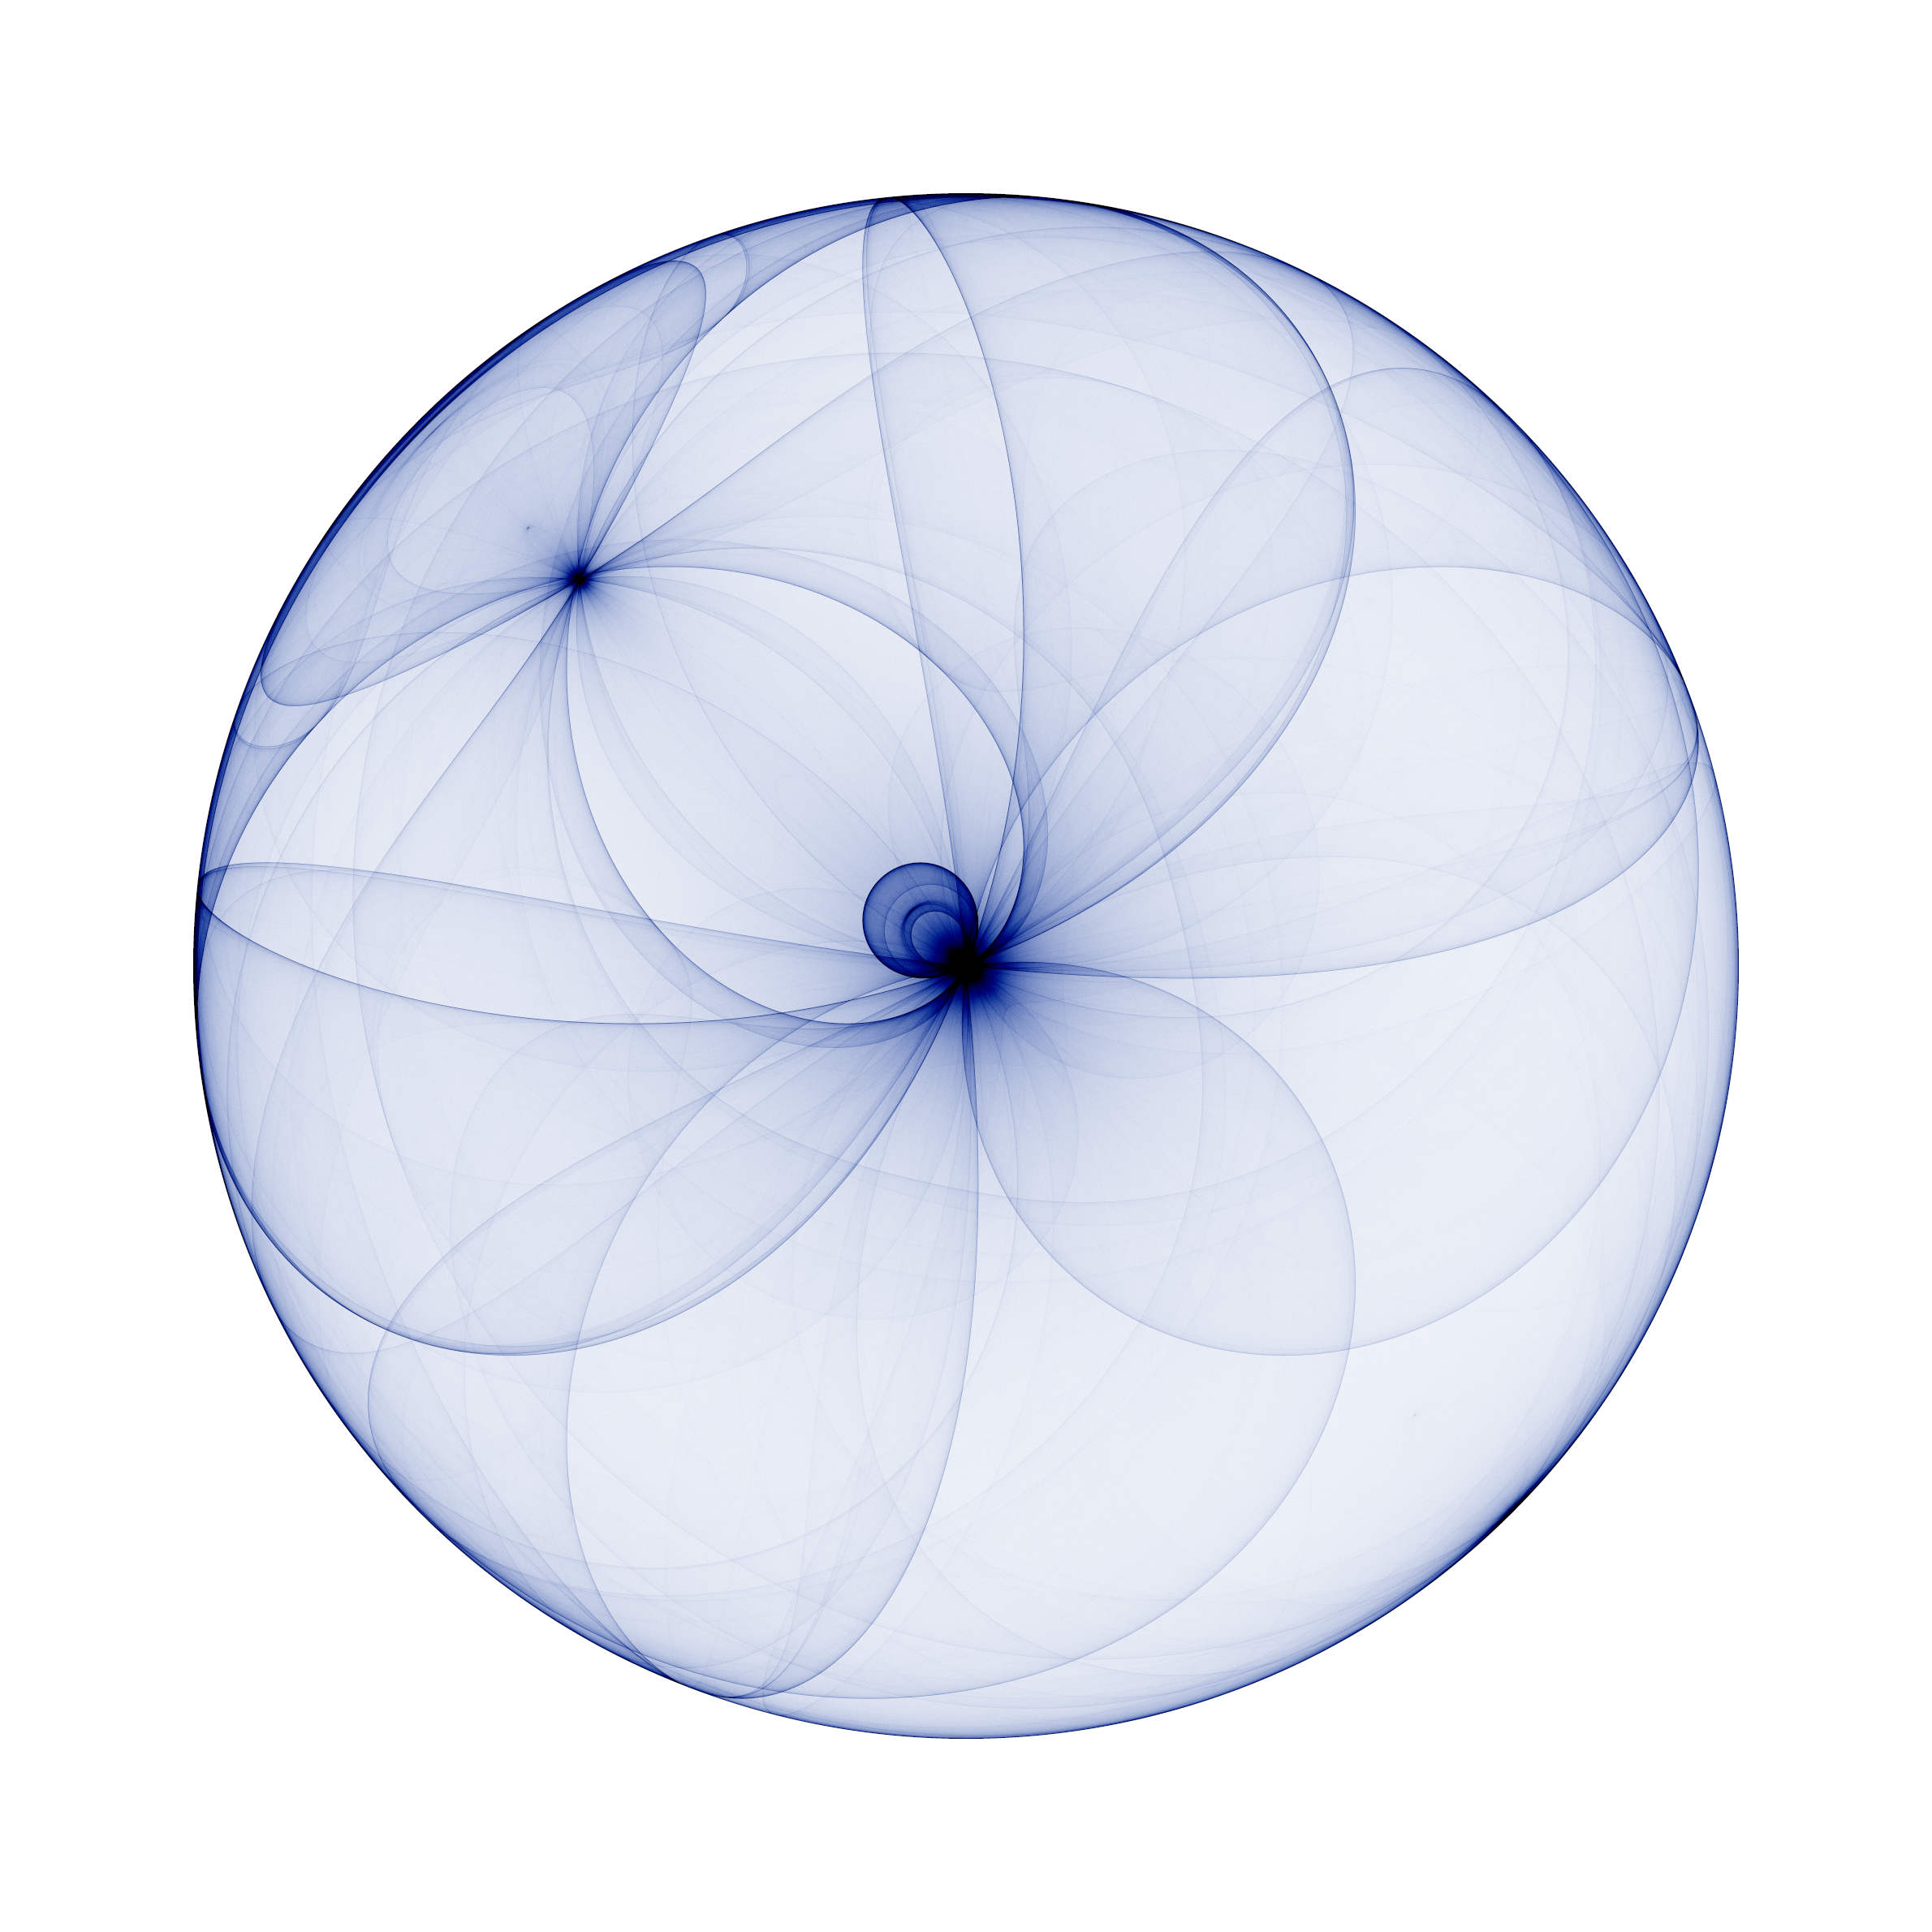
\includegraphics[width=8in]{images/increased-exposure-large.png}
}

%%% increased gamma
\put(17,15){
  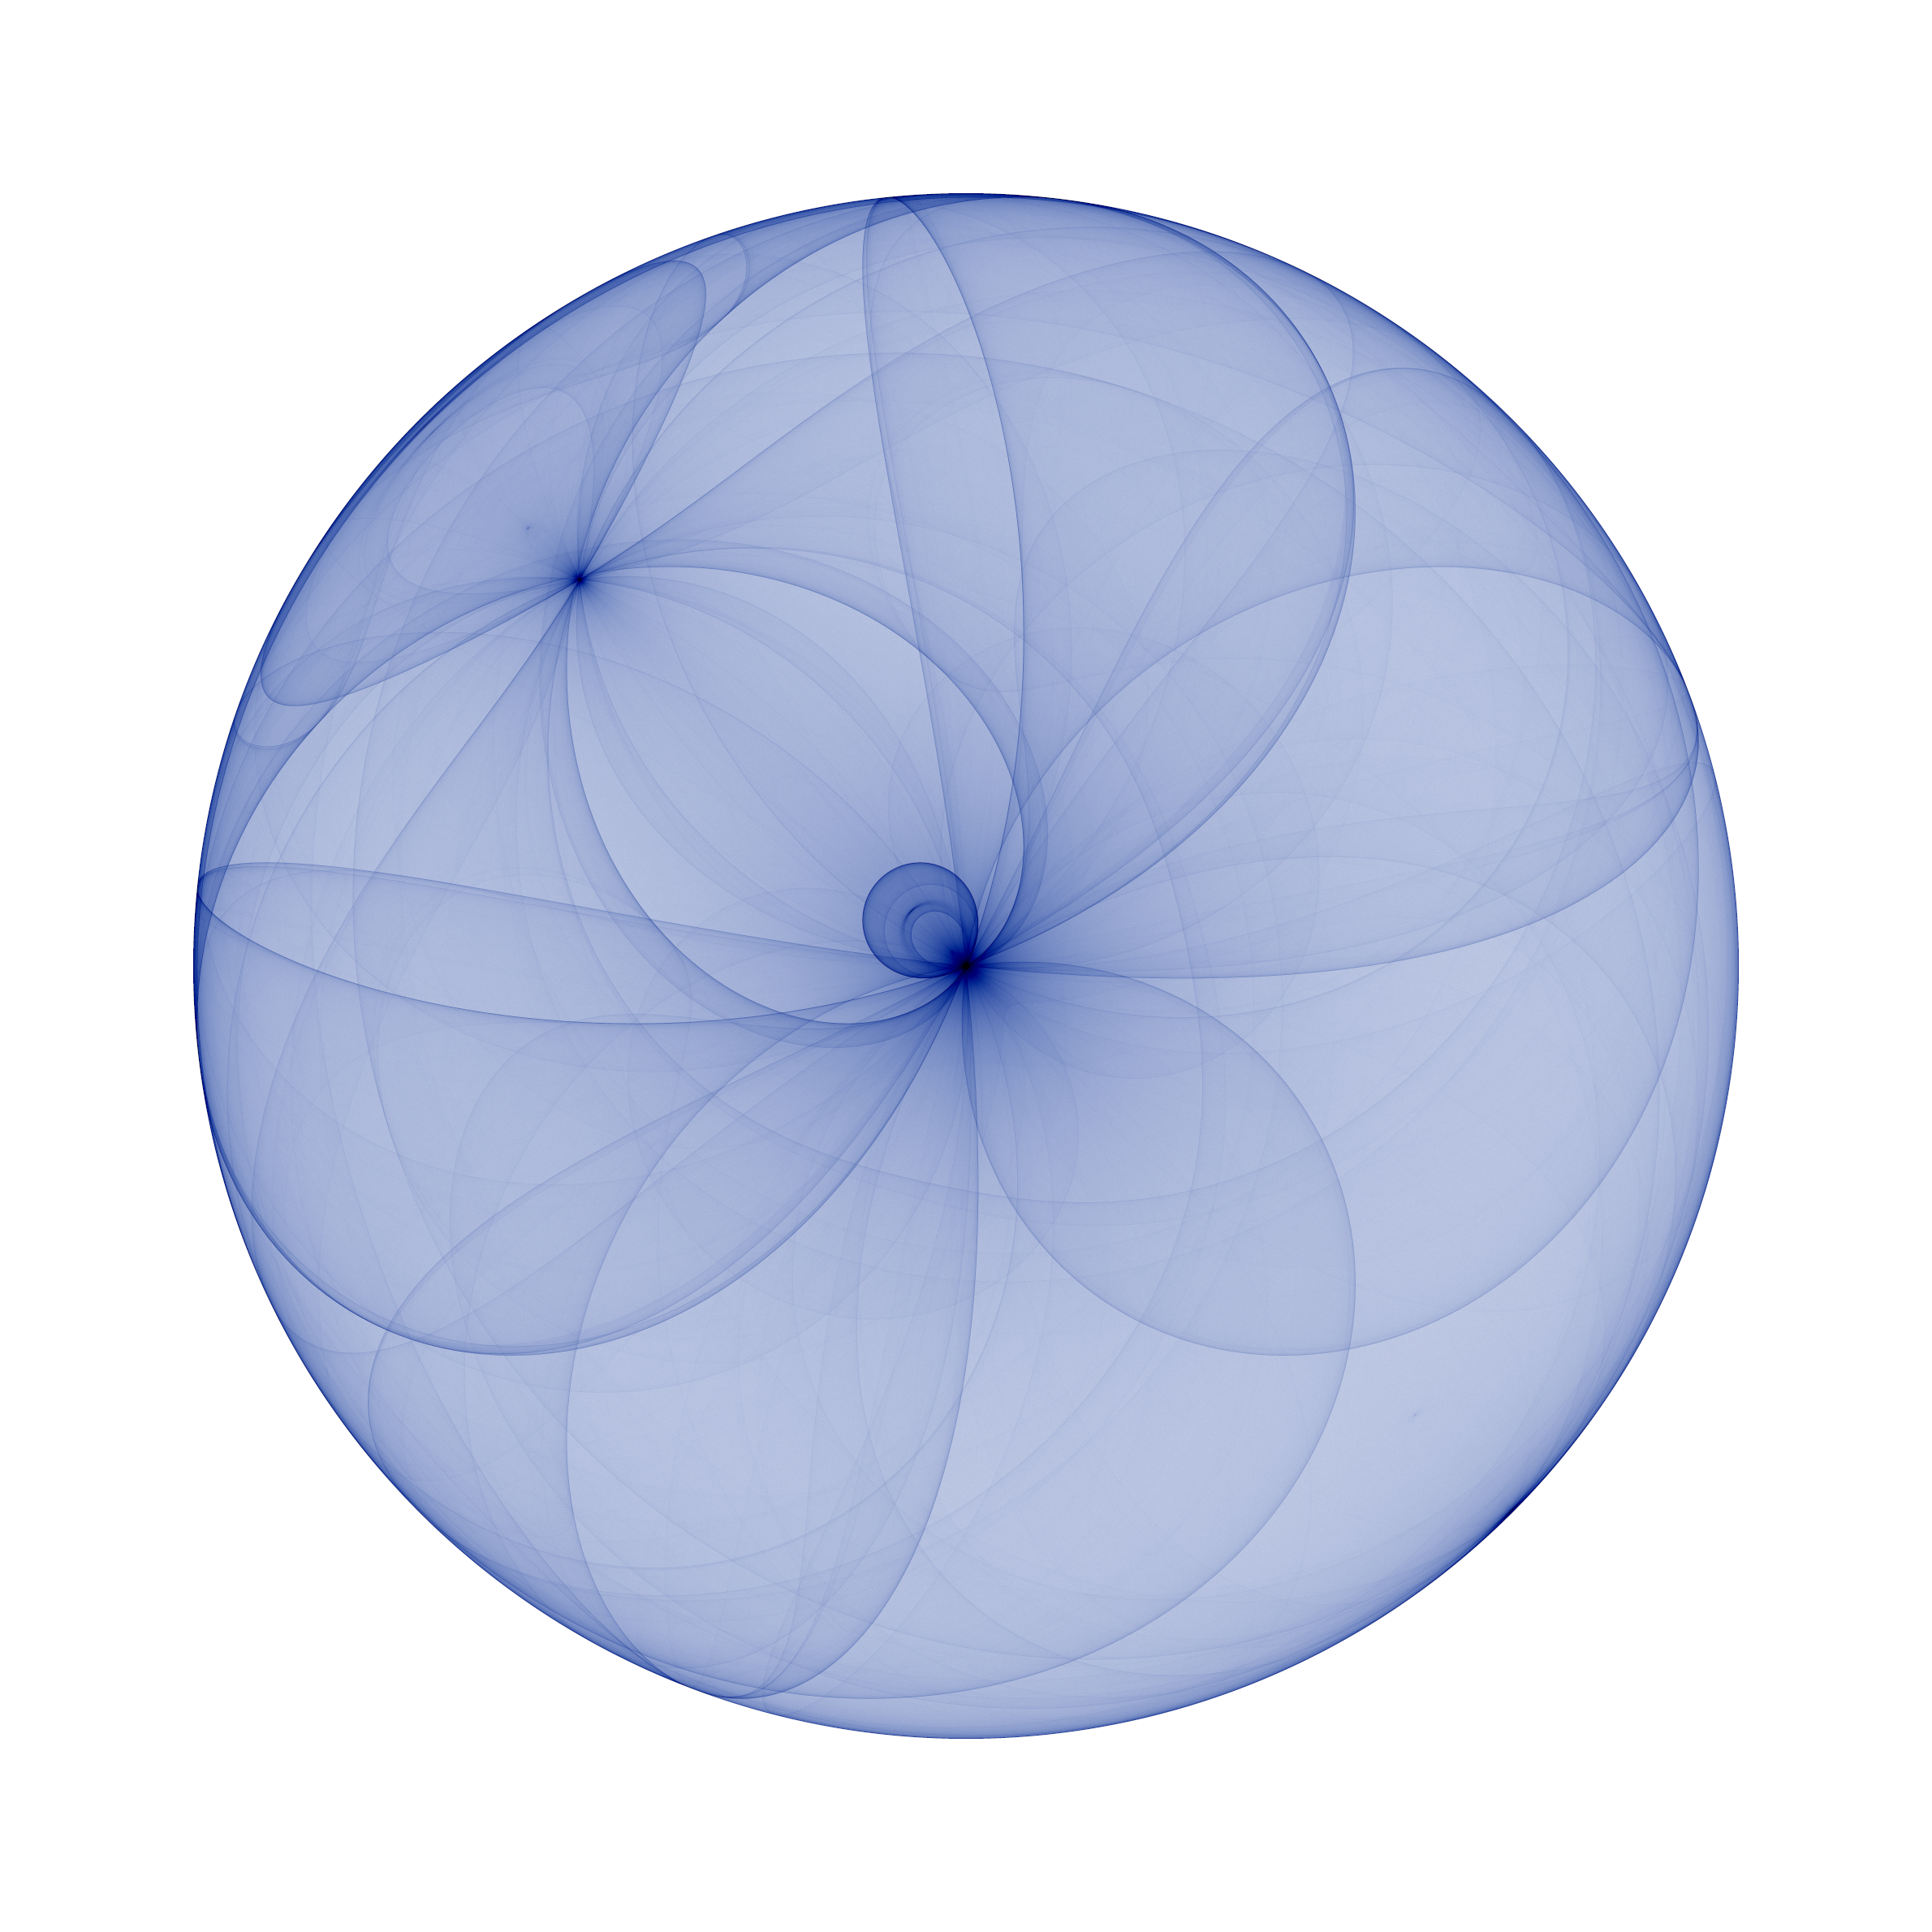
\includegraphics[width=8in]{images/increased-gamma-large.png}
}

%%% decreased exposure, increased gamma
\put(25.5,15){
  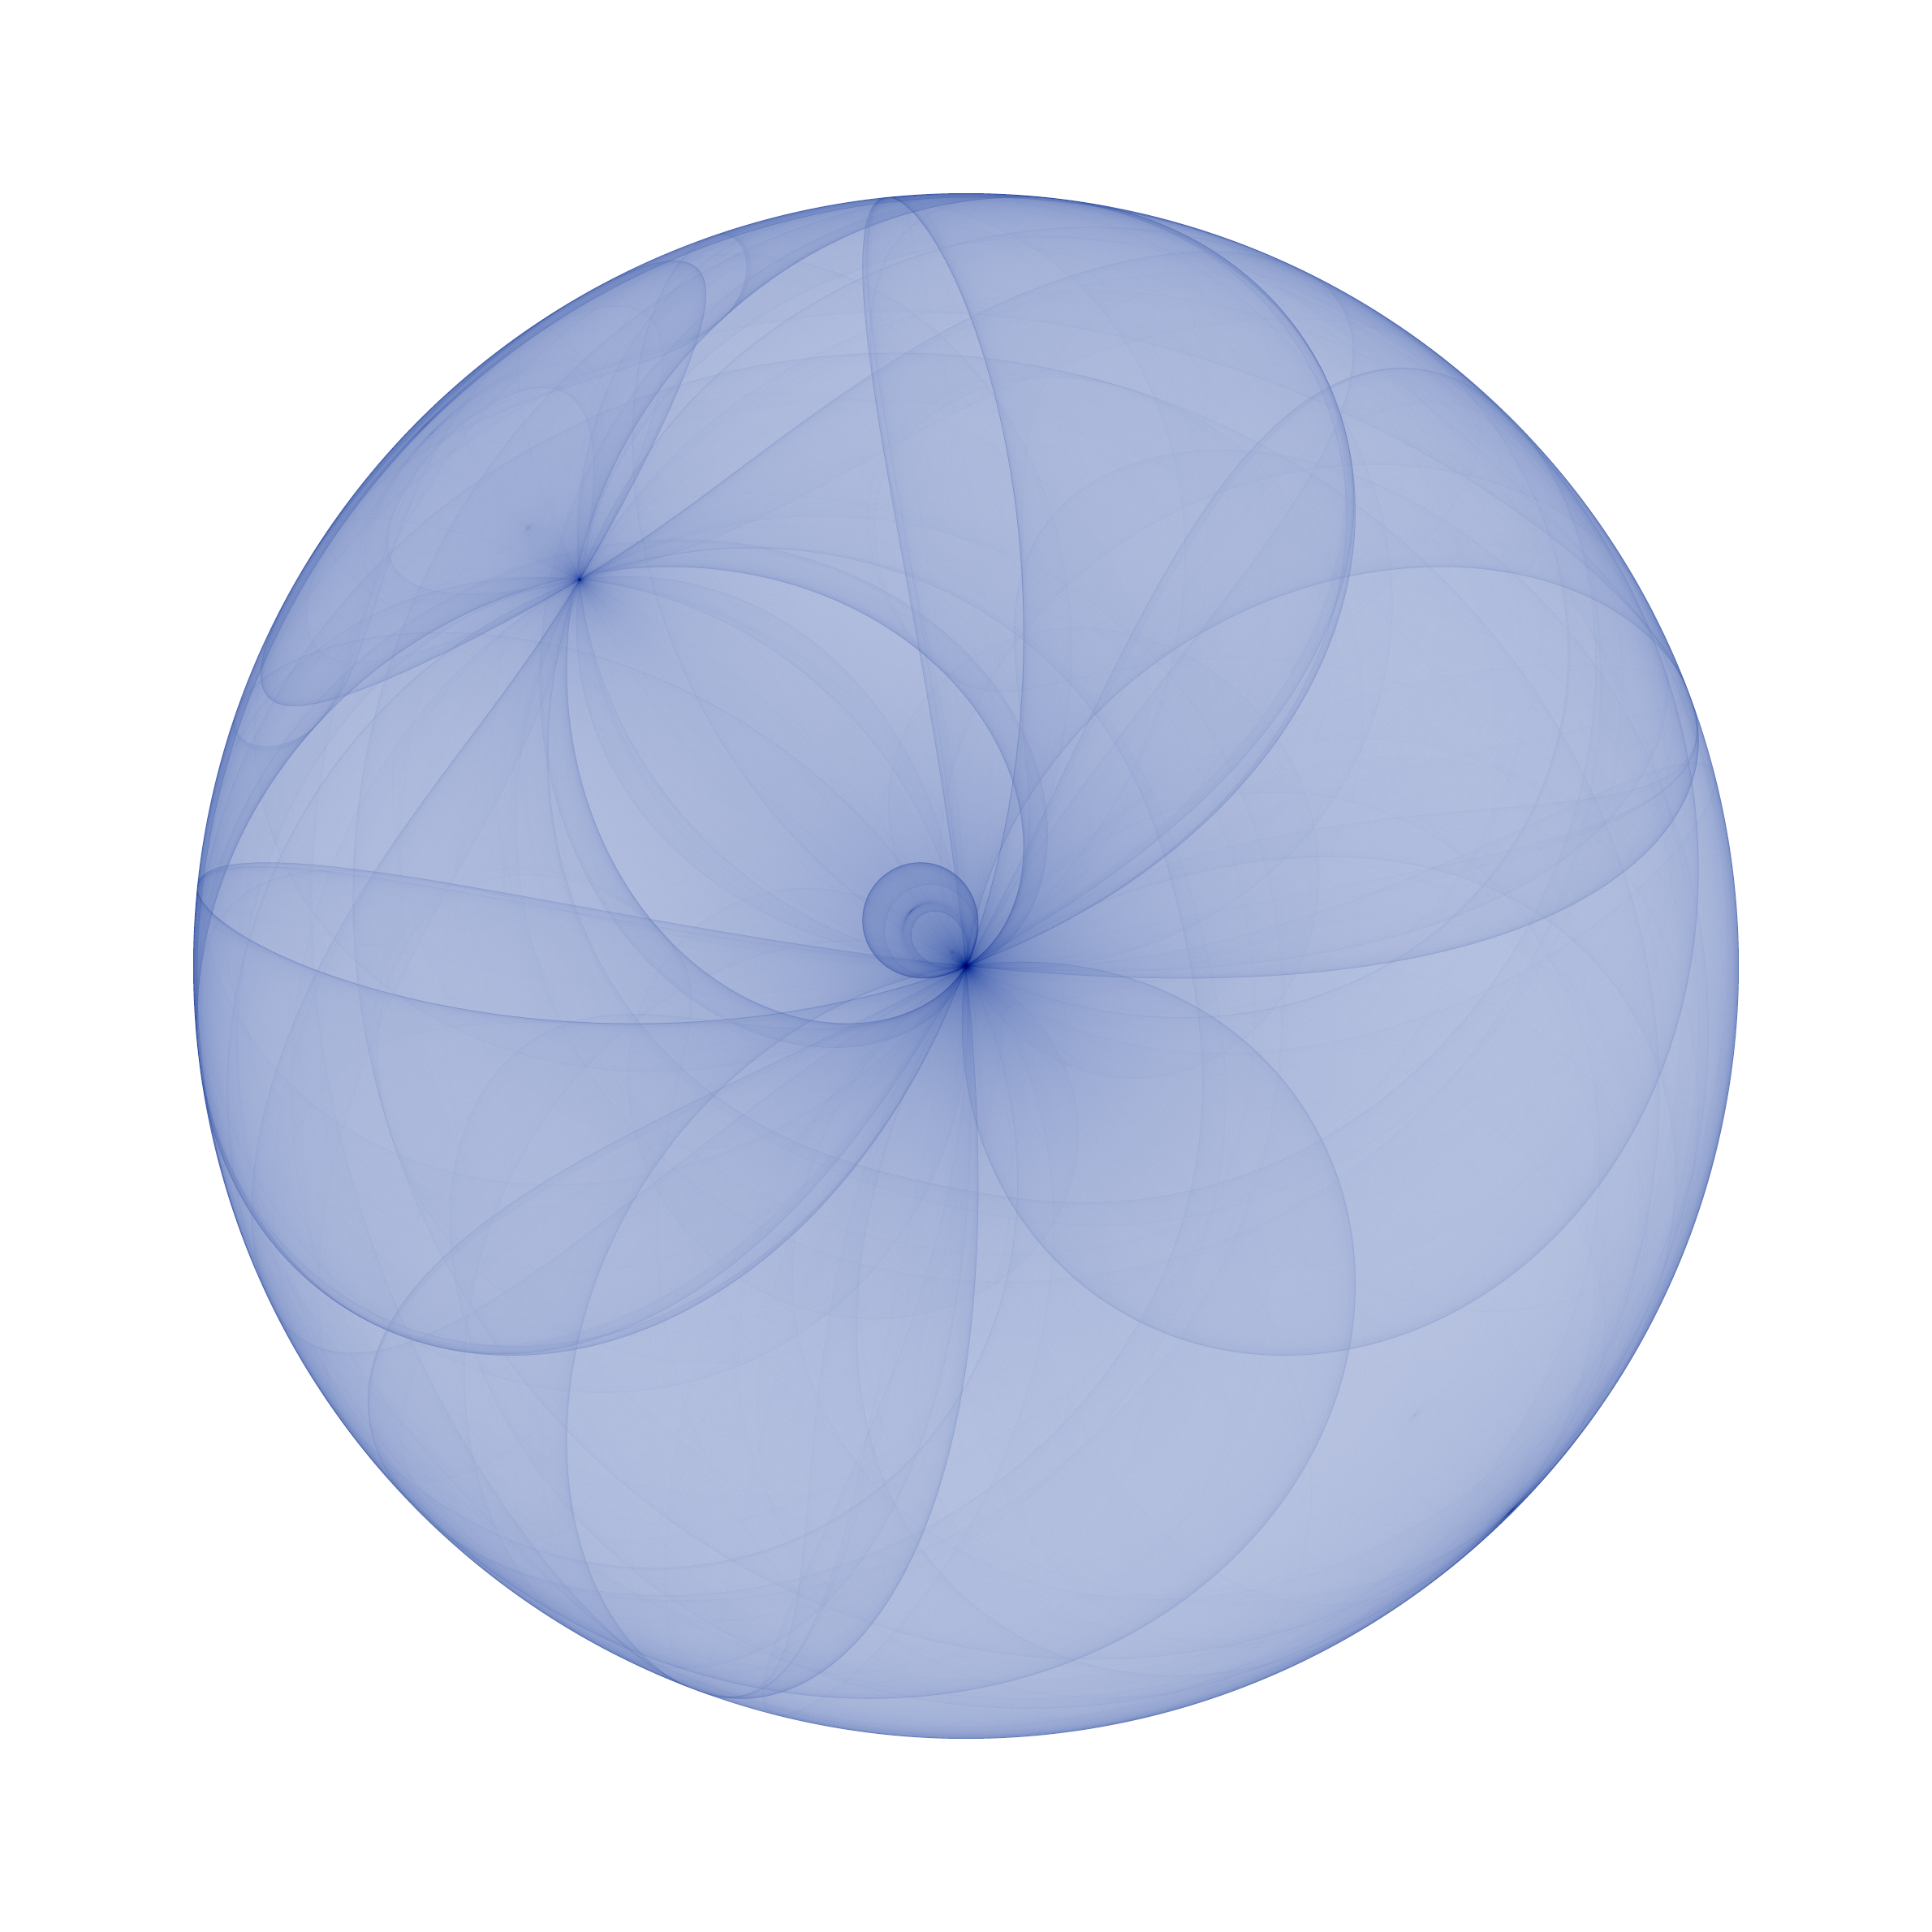
\includegraphics[width=8in]{images/decreased-exposure-increased-gamma-large.png}
}

\end{picture}

\end{document}
